\documentclass[../INDE315.tex]{subfiles} 
\usepackage{fancyhdr}
\usepackage{graphicx}
\usepackage{amsmath}
\usepackage{mhchem}
\usepackage{amssymb}
\usepackage[margin=1in]{geometry}

\graphicspath{{./images/}}

\title{UW IND E 315 Notes}
\author{Anthony Le}

\begin{document}

\pagestyle{fancy}
\fancyhead{}
\fancyhead[R]{UW IND E 315}
\fancyhead[L]{Anthony Le}

\fancyhead[C]{Chapter 2 - Introduction to Probability}

\section*{Chapter 2 - Introduction to Probability}
\subsection*{Simple Example}
\begin{exmp}
    What is the probability of getting heads on the toss of a coin?
\end{exmp}
\begin{defn}
    \textbf{Probability} \\
    The likelihood of a particular outcome/event.
    \begin{enumerate}
        \item Formally: a number from the interval [0,1] to indivate the low (0) to high (1) likelihood of occurrence.
    \end{enumerate}
\end{defn}

\begin{defn}
    \textbf{Sample Space} \\
    The set of all possible outcomes of a random experiment.
    \begin{enumerate}
        \item Event: Subset of the sample space
    \end{enumerate}
\end{defn}

\subsection*{Sample Space and Events (2.1)}
    \begin{center}
        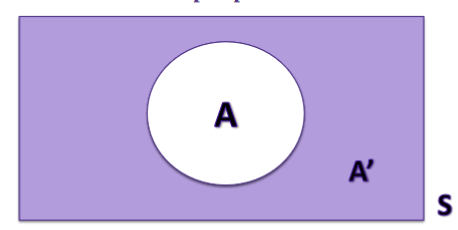
\includegraphics[width = 5cm]{Example2.1}
    \end{center}
Given a sample space $S$ where the probability of S is 1, you can find the probability of event $A$ by subtracting the probability of $A'$ from the probability of the sample space. Describing this in math terms:
\begin{equation*}
    \begin{aligned}
        \text{Sample Space where } P(S) = 1 \\
        P(A) = 1- P(A')
    \end{aligned}
\end{equation*}

\begin{exmp}
    What is the example space for the sum of 2 dice?
\end{exmp}
\begin{equation*}
    \begin{aligned}
        S = {2,3,4,5,6,7,8,9,10,11,12}
    \end{aligned}
\end{equation*}
\begin{enumerate}
    \item Let A be the event that the dice rolls an even number:
        \begin{equation*}
            \begin{aligned}
                A = {2,4,6,8,10,12}
            \end{aligned}
        \end{equation*}
    \item Let B be the event that the dice rolls a prime number:
        \begin{equation*}
            \begin{aligned}
                B = {2,3,5,7,11}
            \end{aligned}
        \end{equation*}
\end{enumerate}
From this, find these following:
\begin{enumerate}
    \item $P(A) = ?$
    \item $P(B) = ?$ 
    \item $P(A|B) = ?$
\end{enumerate}

Here's a graphic showing the sample space for the above situation:
    \begin{center}
        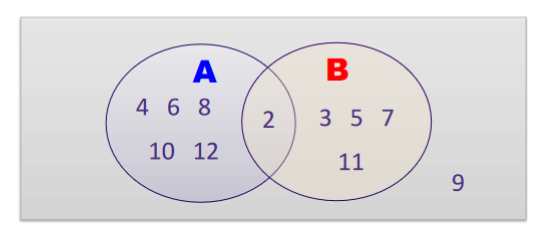
\includegraphics[width = 5cm]{Ch2Example2}
    \end{center}
To find $P(A|B)$:
\begin{equation*}
    \begin{aligned}
        P(A|B) = \frac{P(A \cap B)}{P(B)}
    \end{aligned}
\end{equation*}

\subsubsection*{Interpretations and Axioms of Probability (2.3)}
\begin{enumerate}
    \item Let S be the sample space of some random experiment.
    \item Let E be some event within that sample space.
    \item $P(E)$, the probability of the event is \emph{assigned} based on our knowledge of the system under study.
    \item \emph{Mathematically}, $P(E)$ should satisify the three axioms of probability.
        \begin{enumerate}
            \item The axioms ensure that:
                \begin{enumerate}
                    \item The assigned probabilities can be \emph{interpreted as relateive frequencies}
                    \item The assignments are \emph{consistent with our intuitive understanding} of relationships between relative frequencies.
                \end{enumerate}
        \end{enumerate}
\end{enumerate}

\subsubsection*{Axioms of Probability}
\begin{enumerate}
    \item $0 <= P(E) <= 1$ for any event E.
    \item $P(S) = 1$ where $S$ is the sample space.
    \item If $E_1$, $E_2$,... are mutually exclusive events (ex $E_1 \cap E_2 = 0$), then $P(E_1 \cup E_2) = P(E_1) + P(E_2)$.
\end{enumerate}

\subsubsection*{Event: subset of the sample space - combination of events}
%tags - tag vs cup, union, intersection
\begin{enumerate}
    \item Union of two events
        \begin{enumerate}
            \item All events that are contained in \emph{either} of the two events
            \item Own words - Look at events are in event 1 \emph{or} event 2
            \item Denoted at $E_1 \cup E_2$
        \end{enumerate}
        \begin{center}
            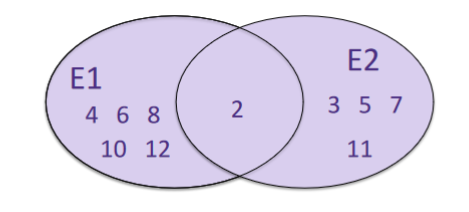
\includegraphics[width = 5cm]{Ch2Event_Union} %//TODO - Consider looking into a way to have this be in line with the text, to the right (maybe using the wrapfig package?)
        \end{center}
    \item Intersection of two events
        \begin{enumerate}
            \item All events that are contained in \emph{both} of the two events
            \item Own words - Look at events that are in event 1 \emph{and} event 2
            \item Denoted as $E_1 \cap E_2$
        \end{enumerate}
        \begin{center}
            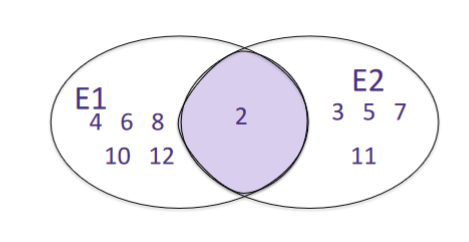
\includegraphics[width = 5cm]{Ch2Event_Intersection}
        \end{center}
    \item Complement of an event
        \begin{enumerate}
            \item All events that are not in the event.
            \item Own words - Look at all events that are \emph{not} in events 1 and 2, but still in the sample space
            \item Denoted as $(E_1 \cup E_2)'$ \footnote{Also note that $((E_1 \cup E_2)')' = E_1 \cup E_2$}
        \end{enumerate}
        \begin{center}
            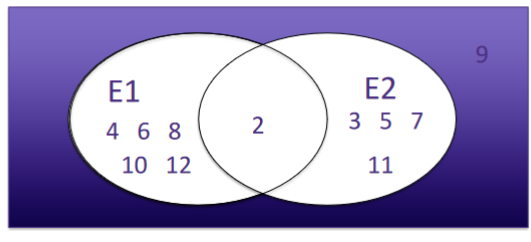
\includegraphics[width = 5cm]{Ch2Event_Complement}
        \end{center}
    \item Mutually Exclusive Events
        \begin{enumerate}
            \item Events share no common outcomes, AKA the occurrence of one event precludes the occurrence of the other.
            \item Denoted as $A \cap B = 0$ 
            \item Example - not being able to roll a head and a tail on a coin at the same time.
        \end{enumerate}
        \begin{center}
            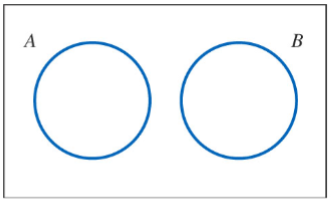
\includegraphics[width = 5cm]{Ch2Event_MutuallyExclusive}
        \end{center}
\end{enumerate}

\subsection*{Counting Techniques (2.2)}
\begin{enumerate}
    \item Now we have built the conceptual framework of probability.
    \item To apply this framework to solve real-world problems, we still need methods. 
    \item We'll first learn three counting techniques:
        \begin{enumerate}
            \item Multiplication rule
            \item Permutation rule
            \item Combination rule
        \end{enumerate}
\end{enumerate}

\subsubsection*{Multiplication Rule}
\begin{defn}
    \textbf{Multiplication Rule}
    \begin{enumerate}
        \item Let an operation consist of $k$ steps and \dots 
            \begin{enumerate}
                \item $n_1$ ways of completing step 1, 
                \item $n_2$ ways of completing step 2, (repeat until you reach step k)
                \item $n_k$ ways of completing step $k$.
            \end{enumerate}
        \item From this, the total number of ways or outcomes are:
            \begin{enumerate}
                \item $n_1 * n_2 * \dots * n_k$
            \end{enumerate}
    \end{enumerate}
\end{defn}


\begin{exmp}
    A message is recieved either on time or late. If we were to receive three messages, what are all the possible results for the three messages?
    \begin{center}
        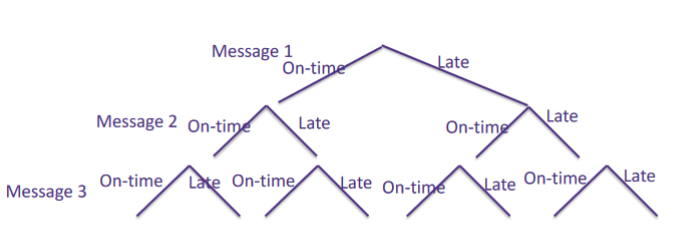
\includegraphics[width = 5 cm]{Ch2Example3}
    \end{center}
\end{exmp}
\begin{equation*}
    \begin{aligned}
        2 * 2 * 2 = 8 \quad \text{possible results}
    \end{aligned}
\end{equation*}
Another example:
\begin{exmp}
    With 4 colors, 3 fonts, and 3 image positions available for a website, how many different designs are possible? 
\end{exmp}
\begin{equation*}
    \begin{aligned}
        4 * 3 * 3 = 36 \quad \text{possible designs}
    \end{aligned}
\end{equation*}

\subsubsection*{Permutation Rule}
\begin{enumerate}
    \item If the sample space contains 3 items, $S = {a, b, c}$ 
    \begin{enumerate}
        \item Then there are 6 permutations (or 3!)
        \item abc, acb, bac, bca, cab, cba \emph{(order matters)}
        \item This represents the number of ways 3 people can be rearranged
    \end{enumerate} 
\end{enumerate}
\begin{defn}
    \textbf{Permutation Rule}
    \begin{enumerate}
        \item A permutation is a unique sequence of distinct items. 
        \item The number of permutations for a set of $n$ items is $n!$
            \begin{enumerate}
                \item Not sequencing any items, we get that:
                    \begin{equation*}
                        \begin{aligned}
                            P^n = n!
                        \end{aligned}
                    \end{equation*}
                \item To sequence only $r$ items from a set of $n$ \emph{different} items:
                    \begin{equation*}
                        \begin{aligned}
                            P^n_r = \frac{n!}{(n-r)!}
                        \end{aligned}
                    \end{equation*}
                \item To sequence only $r$ items from a set of $n$ \emph{identical} items:\footnote{Where $n = n_1 + n_2 + \dots n_r$  identical items}
                    \begin{equation*}
                        \begin{aligned}
                            P^n_r = \frac{n!}{n_1! n_2! \dots n_r!}
                        \end{aligned}
                    \end{equation*}

            \end{enumerate}
    \end{enumerate}    
\end{defn}

For example:
\begin{exmp}
    Sequence only 3 items from a set of 7 items.
\end{exmp}
\begin{equation*}
    \begin{aligned}
        P^7_3 &= \frac{7!}{(7-3)!} \\
                &= \frac{7!}{4!} \\
                &= \frac{7X6X5X4!}{4!} \\
                &= 210
    \end{aligned}
\end{equation*}
Another example:
\begin{exmp}
    Say we have 4 locations, and we want to place 2 different components on those locations. How many different sequences will we have?
\end{exmp}
In other words, sequence 2 locations from a set of 4 locations.
\begin{equation*}
    \begin{aligned}
        P^4_2 = &= \frac{4!}{(4-2)!} \\
                &= \frac{4*3*2*1}{2*1} \\
                &= 12
    \end{aligned}
\end{equation*}

%To sequence permutations of similar objects
%\begin{enumerate}
%    \item Used for counting the sequences when not all the items are different.
%    \item Where the number of permutations of n where:
%        \begin{enumerate}
%            \item $n_1$ are identical,
%            \item $n_2$ are identical, ..., and
%            \item $n_r$ are identical
%        \end{enumerate}
%    \item Is calculated as:
%        \begin{equation*}
%            \begin{aligned}
%                \frac{n!}{n_1! n_2! \dots n_r!}
%            \end{aligned}
%        \end{equation*}
%\end{enumerate}

\begin{exmp}
    A hospital operating room needs to schedule three knee surgeries and
    two hip surgeries in a day. The number of possible sequences of three knee and two hip surgeries is:
\end{exmp}
\begin{equation*}
    \begin{aligned}
        n &= 2 + 3 = 5 \\
        P^5 &= \frac{n!}{n_1! n_2! \dots n_r!} \\
            &= \frac{5!}{2!3!} \\
            &= 10
    \end{aligned}
\end{equation*}

\subsubsection*{Combination Rule}
\begin{defn}
    \textbf{Combination Rule}
    \begin{enumerate}
        \item A combination is a selection of $r$ items from a set of $n$ where \emph{their order doesn't matter.}\footnote{Since order doesn't matter you could also look at combinations as whether a solution HAS the items you're looking for. Think for S = {a,b,c}, we found multiple permutations for r = 3. However, as we'll see, we only get 1 \emph{combination} for r = 3}
        \item If $S = {a,b,c}$,
            \begin{enumerate}
                \item If $r = 3$, there is only 1 combination - $abc$\footnote{Think about this as there only being one solution where the solution contains 3 items!}
                \item If $r = 2$, there are 3 combinations - $ab$, $ac$, $bc$
            \end{enumerate}
            \begin{equation*}
                \begin{aligned}
                    C^n_r = \left( \begin{tabular}{c}
                        n \\
                        r
                        \end{tabular}  \right) = \frac{n!}{r!(n-r)!} 
                \end{aligned}
            \end{equation*}
        \item \textbf{Note} - the number of permutations $>=$ the number of combinations \textbf{always}
    \end{enumerate}
\end{defn}

For example:
\begin{exmp}
    A circuit board has 8 possible locations. If 5 \emph{identical} components are to be placed on a board, how many different designs are possible?
\end{exmp}
Since the components are identical, order doesn't matter, making the combination rule ideal for this. Using the combination rule:
\begin{equation*}
    \begin{aligned}
        C^8_5 &= \frac{8!}{5!(8-5)!} \\
                &= \frac{8*7*6*5!}{5!*3*2*1} \\
                &= 56
    \end{aligned}
\end{equation*}
Checking that number of permuations is greater/equal to number of combinations:
\begin{equation*}
    \begin{aligned}
        P^8_5 = 6,720 \quad C^8_5 = 56
    \end{aligned}
\end{equation*}

Recapping what we've learned so far, we learned 3 counting techniques:
\begin{enumerate}
    \item Multiplication rule (steps)
    \item Permutation rule (different elements)
    \item Combination rule (same elements)
\end{enumerate}
These 3 rules can be used in combination to address more difficult questions, such as sampling with or without replacement.

\subsubsection*{Sampling without replacement}
\begin{exmp}
    A bin of 50 parts contains 3 defectives and 47 good parts. A sample of 6 parts is selected from the 50 without replacement. \\
    How many different samples of size 6 are there that contain EXACTLY 2 defective parts? \\
    OR \\
    How many different samples of size 6 are there that contain exactly 4 hood parts?
\end{exmp}
\begin{enumerate}
    \item Step 1
        \begin{enumerate}
            \item How many possible ways are there of getting exactly 2 defects when there are only 3?
            %\item Even though the problem asks for a sample size of 6, we can get away with only looking at the 3 defectives and finding the number of combinations to get the defectives(?)
            \item I think we have to start with looking at the step of selecting defective and good parts from the sample space itself, then applying those numbers to the sample size of 6
                \begin{equation*}
                    \begin{aligned}
                        C^3_2 &= \frac{n!}{r!(n-r)!} \\
                                &= \frac{3!}{2!1!} \\
                                &= 3 \quad \text{different ways}
                    \end{aligned}
                \end{equation*}
        \end{enumerate}
    \item Step 2
        \begin{enumerate}
            \item How many ways are there of selecting 4 good parts from the 47 acceptable parts?
            \item Like what we have done for the defect parts, we look at the combinations of selecting acceptable parts from the sample space first.
                \begin{equation*}
                    \begin{aligned}
                        C^{47}_4 &= \frac{n!}{r!(n-r)!} \\
                                    &= \frac{47!}{4!(47-4)!} \\
                                    &= \frac{47!}{4!43!} \\
                                    &= 178,365 \quad \text{different ways}
                    \end{aligned}
                \end{equation*} 
        \end{enumerate}
    \item Step 3
        \begin{enumerate}
            \item Apply the multiplication rule
            \item Once we have found the combinations for defective and acceptable parts, we can now apply the sample size of 6 constraint
            \item From the original problem, how many possible ways are there of getting exactly 2 of 3 defectives AND 4 from the 47 acceptable parts?
                \begin{equation*}
                    \begin{aligned}
                        C^3_2 C^{47}_4 &= 3 * 178,365 \\
                                    &= 535,095 \quad \text{different ways}
                    \end{aligned}
                \end{equation*}     
        \end{enumerate}
    \item Step 4
        \begin{enumerate}
            \item What is the probability of this event occurring?
            \item First, we find the total number of ways to select 6 parts (of any type) out of the 50 parts.
                \begin{equation*}
                    \begin{aligned}
                        C^{50}_6 &= \frac{n!}{r!(n-r)!} \\
                                &= \frac{50!}{6!(50-6)!} \\ 
                                &= \frac{50!}{6!44!} \\
                                &= 15,890,700
                    \end{aligned}
                \end{equation*}
            \item Then, we find the probability by dividing the combinations of getting 2 defects by total combinations.
                \begin{equation*}
                    \begin{aligned}
                        P(2\text{ defects}|\text{Sample of }6) &= \frac{C^3_2 C^{47}_4}{C^{50}_6} \\
                                &= \frac{535,095}{15,890,700} \\
                                &= 0.034
                    \end{aligned}
                \end{equation*}
        \end{enumerate}
\end{enumerate}
Notes regarding the previous example - we multiplied $C^3_2 C^{47}_4$ together as they are dependent on each other; one event can't happen without the other. What this means in the case of this problem is that when we select 2 defectives to be in our sample size of 6, we must then have 4 good parts in the 6 selected!

\subsection*{Addition Rules}
\begin{enumerate}
    \item Probabilities of joint events can often be determined from the probabilities of the individual events that comprise it.
        \begin{enumerate}
            \item Probability of a union:
                \begin{equation*}
                    \begin{aligned}
                        P(A \cup B) = P(A) + P(B) - P(A \cap B) 
                    \end{aligned}
                \end{equation*}
            \item Probability of a intersection:
                \begin{equation*}
                    \begin{aligned}
                        P(A \cap B) = P(A) + P(B) - P(A \cup B) 
                    \end{aligned}
                \end{equation*}
            \item However, if events A and B are mutually exclusive, then:
                \begin{equation*}
                    \begin{aligned}
                        & P(A \cap B) &= 0, \\
                        \therefore & P(A \cup B) &= P(A) + P(B)
                    \end{aligned}
                \end{equation*}
        \end{enumerate}
\end{enumerate}

%//TODO - include semiconductor wafer example here!

\subsection*{Conditional Probability (2.5)}
\begin{enumerate}
    \item Probabilties may need to be reevaluated as additional information becomes available.
    \item P(B|A) is called the the probability of event B occurring, given that event A has already occurred. Example questions could be:
        \begin{enumerate}
            \item What is the probability that UW will win the next football game, \emph{given that} it won the last game?
            \item What is the probability that the letter 'a' will be typed \emph{given that} 'for ex' was typed on Google Search?
        \end{enumerate}
\end{enumerate}

\begin{defn}
    \textbf{Conditional Probability Rule} \\
    The conditional probability of event $B$ given event $A$, denoted as $P(B|A)$, is: 
        \begin{equation*}
            \begin{aligned}
                P(B|A) = P(A \cap B) / P(A) \quad \text{for} \quad P(A) > 0 
            \end{aligned}
        \end{equation*}
    \emph{Therefore}, $P(B|A)$ can be viewed as the relative frequency of event B among the trials that produce an outcome in event A. 
\end{defn}

\subsection*{Multiplication Rule for Probabilities (2.6)}
The conditional probability can be rewritten to provide the multiplication rule.
    \begin{equation*}
        \begin{aligned}
            P(A \cap B) &= P(B|A) * P(A) \\
                    &= P(A|B) * P(B) \\
        \end{aligned}
    \end{equation*} 
This gives you the probability of the intersection of two events.

\subsection*{Total Probability Rule (2.6)}
For any two events $A$ and $B$:
    \begin{equation*}
        \begin{aligned}
            P(B) &= P(B \cap A) + P(B \cap A') \\
                &= P(B|A) * P(A) + P(B|A') * P(A')
        \end{aligned}
    \end{equation*} 

\subsection*{Independence (2.7)}
\begin{defn}
    \textbf{Independence} \\
    Where the occurrence of one event has no impact on the occurrence of the other event.
    \begin{enumerate}
        \item Two events are independent if the following equivalent statements are true:
            \begin{enumerate}
                \item $P(A|B) = P(A)$
                \item $P(B|A) = P(B)$
                \item $P(A \cap B) = P(A)P(B)$
            \end{enumerate}
    \end{enumerate}
\end{defn}

\subsubsection*{Example - Independence}
\begin{enumerate}
    \item Consider a fair coin and a fair six-sided dice.
    \item Event A is obtaining heads and Event B is rolling a 6.
    \item We can reasonable assume that events A and B are independent and therefore don't effect the outcome of each other.
        \begin{enumerate}
            \item With this assumption, the probability that both A and B occur is
                \begin{equation*}
                    \begin{aligned}
                        P(A \cap B) &= P(A) P(B) \\
                                &= (1/2) (1/6) \\
                                &= 1/12
                    \end{aligned}
                \end{equation*} 
        \end{enumerate}
\end{enumerate}

\subsubsection*{Example - Mutually Exclusive Independence}
\begin{enumerate}
    \item Consider a fair six-sided dice as before, only in addition to the numbers 1 through 6 on each face, we have the property that:
        \begin{enumerate}
            \item Even-numbered faces are colored red
            \item Odd-numbered faces are colored green
        \end{enumerate}
    \item Event A is rolling a green face
    \item Event B is rolling a 6
    \item The probability of events A and B occurring at the same time (or $P(A \cap B)$) is 0, since the events are mutually exclusive.
\end{enumerate}

\subsection*{DeMorgan's Law}
\begin{enumerate}
    \item Finding the compliements of the union or the intersection of two events:
        \begin{equation*}
            \begin{aligned}
                (A \cap B)' &= A' \cup B' \\
                (A \cup B)' &= A' \cap B' \\
            \end{aligned}
        \end{equation*}
\end{enumerate}

\subsubsection*{Example - 2-23}
\begin{exmp}
    Series Circuit - the following circuit operates only if there is a path of functional devices from left to right. The probability that each device functions is shown on the graph. Assume the devices fail independently. What is the probability that the circuit operates?
    \begin{center}
        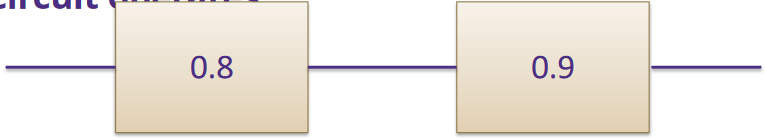
\includegraphics[width = 5cm]{Ch2Example4}
    \end{center}
\end{exmp}
\begin{enumerate}
    \item Since the circuit requires both devices to function due to being a series circuit, to determine the probability that the circuit operates, find the chance of the left AND right devices functioning:
        \begin{equation*}
            \begin{aligned}
                P(\text{L AND R}) &= P(L \cap R) \\
                        &= P(L) P(R) \\
                        &= (0.8)(0.9) \\
                        &= 0.72
            \end{aligned}
        \end{equation*}
\end{enumerate}

\subsubsection*{Example 2-24}
\begin{exmp}
    Parallel Circuit - The following circuit operates only if there is a path of functional devices from left to right. The propability that each device functions is shown on the graph. Assume the devices fail independently. What is the probability that the circuit operates?
    \begin{center}
        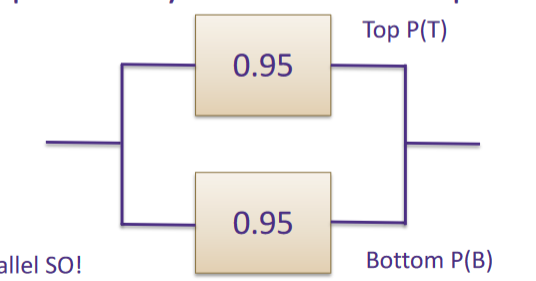
\includegraphics[width = 5cm]{Ch2Example5}
    \end{center}
\end{exmp}
\begin{enumerate}
    \item This problem uses similar logic to the previous example. However, since this is a parallel circuit, the circuit can still function if the top or bottom devices stop working, as long as there is a functional device. In other words, find the probability of the top device OR bottom device working.
        \begin{equation*}
            \begin{aligned}
                P(\text{T or B}) &= 1 - [P(\text{T or B})'] \\
                                &= 1 - P(\text{T' and B'}) \\
                P(\text{T' and B'}) &= P(T') P(B')  \\
                                    &= (1-0.95)^2 \\
                                    &= 0.05^2 \\
                P(\text{T or B}) &= 1 - P(T') P(B') \\
                                &= 1- 0.05^2 \\
                                &= 0.9975 
            \end{aligned}
        \end{equation*} 
    \item Keep in mind that using the apostrophe (') when finding probability is similar to using a NOT statement (take the inverse)- for example, if P(T) represents the probability of the top device working, P(T') represents the probability of the device FAILING.
\end{enumerate}


\end{document}